\documentclass{article}
\usepackage{mathtools}
\usepackage{float}
\usepackage[margin=1cm]{geometry}
\usepackage{listings}
\usepackage{tikz-qtree}

\tikzset{
    labeled/.style = {
        circle, draw, thick, minimum size=1.5em, inner sep=0, label=right:{#1}
    }
}
\lstset{
    basicstyle=\footnotesize\ttfamily,
    breaklines=false
}

\begin{document}
Dustin Randall \\

\section{RBT}
\subsection*{Invariants}
{\footnotesize
    \begin{itemize}
        \item Root node is black
        \item Red nodes have black parent
        \item All paths to leaf nodes contain same number of black nodes
    \end{itemize}
}
\subsection*{Insert}
Start with normal BST insert, new node is red.
\begin{lstlisting}
    while(z.parent && z.parent.Color == R) {
        if(u(z).Color == R) p(z).Color = B; u(z).Color = B; p(p(z)).Color = R; z = p(p(z));
        else if(p(p(z)) is ZigZag)
            Rotate Parent away from z
            z = old sibling
        else
            swapColors(p(p(z)), p(z))
            Rotate Grandparent away from z
    }
    root.Color = B;
\end{lstlisting}

\subsection*{Delete}
Start with normal BST delete
\begin{lstlisting}
    z = node to delete
    y = (z.Left && z.Right) ? Successor(z) : z
    x = y.Left ? y.Left : y.Right // node is y's place after delete
    y.Color = z.Color;
    if(oldY.Color == R) return;
    while(p(x) && x.Color == B) {
        w = sibling(x)
        if(w.Color == R) swapColors(p(x), w); Rotate p(x) away from w
        else if(w.Left.Color == B && w.Right.Color == B) w.Color = R; x = p(x)
        else if(x.Near.Color == R && x.Far.Color == B) 
            Rotate w away from x; swapColors(w, x.Near)
        else if(x.Far.Color == R) swapColors(p(x), w); Rotate p(x) toward x; x = root
    }
    x.Color = B;
\end{lstlisting}

\section{B-Tree}
\subsection*{Invariants}
{\footnotesize
    \begin{itemize}
        \item All leaf nodes are at same depth
        \item Each node has between \(t-1\) and \(2t-1\) keys (except root)
    \end{itemize}
}
\subsection*{Insert}
If current node is full, Split.
Split: Promote the middle key to the parent node, left and right half become new nodes.
Always insert into a leaf node.

\subsection*{Delete}
Delete(node, key) requires node.Count $>= t$, use Merge to ensure this. \\
Borrow means move the borrowed key up, and the current node down \\
\begin{lstlisting}
if(node is leaf) remove key if found
else {
    n = node.Find(key);
    if(n == key) {
        if(n.Left.Count >= t) {
            pred = Max(n.Left);
            n = pred;
            Delete(n.Left, pred);
        } else if(n.Right.Count >= t) {
            succ = Min(n.Right);
            n = succ;
            Delete(n.Right, succ);
        } else {
            n.Left = Merge(n.Left, n.Right, n);
            Delete(n.Left, key);
        }
    } else {
        if(n.Child.Count < t) {
            if(Left(n).Count >= t) BorrowFromLeft(n);
            else if(Right(n).Count >= t) BorrowFromRight(n);
            else Merge(Left(n), Right(n), n);
            Delete(n.Child, key);
        }
    }
}
\end{lstlisting}

\section{Heaps}
\subsection*{Invariants}
{\footnotesize
    \begin{itemize}
        \item Complete Binary Tree (every level filled except possibly last, filled left to right)
        \item Max-Heap: Parent value $>=$ children values
        \item MaxHeapify: sift-down, swapping with largest child until a heap. \(O(\log h)\)
        \item IncreaseKey: sift-up, swapping with parent until a heap. \(O(\log h)\)
    \end{itemize}
}
\section{Huffman Coding}
Greedy algorithm for lossless data compression. \\
a:40, b:30, c: 90, d: 20, e: 60, f: 120, g:10, h:5 \\
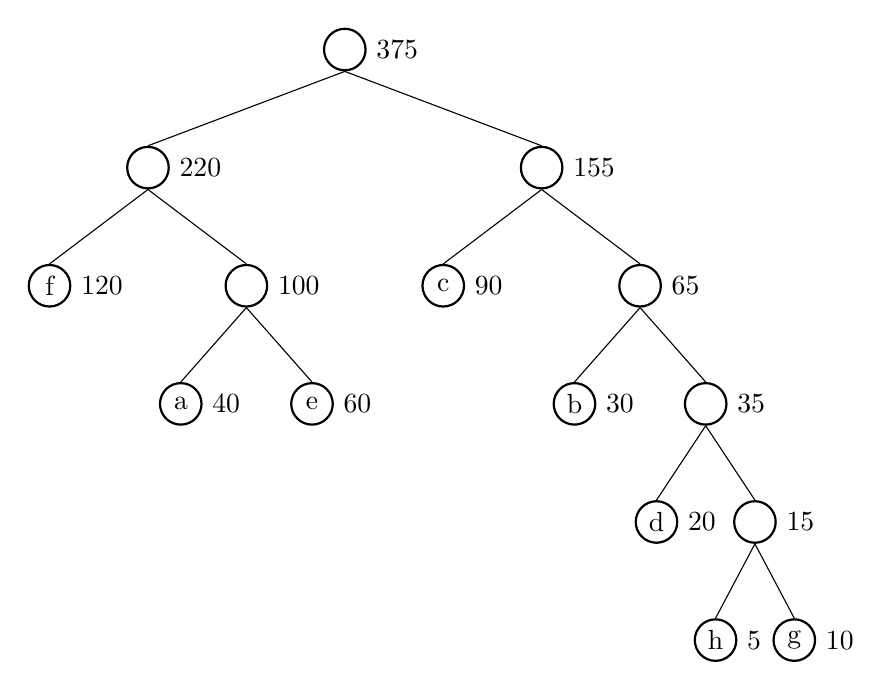
\begin{tikzpicture}[level/.style={sibling distance=50mm/#1}]
    \node[labeled=375]{}
        child {node[labeled=220] {} 
            child {node[labeled=120]{f} }
            child {node[labeled=100]{} 
                child {node[labeled=40]{a} }
                child {node[labeled=60]{e} }
            }
        }
        child {node[labeled=155] {}
            child {node[labeled=90]{c} }
            child {node[labeled=65]{}
                child {node[labeled=30]{b} }
                child {node[labeled=35] {}
                    child {node[labeled=20]{d} }
                    child {node[labeled=15] {}
                        child {node[labeled=5]{h}}
                        child {node[labeled=10]{g}}
                    }
                }
            }
        };
\end{tikzpicture}
\end{document}